\documentclass[10pt,letterpaper]{article}
\usepackage[utf8]{inputenc}
\usepackage{amsmath}
\DeclareMathOperator{\sign}{sgn}
\usepackage{amsfonts}
\usepackage{amssymb}
\usepackage[margin=1in]{geometry}
\usepackage{graphicx}
\usepackage{sidecap}
\usepackage{float}

\title{\vspace{-4ex}Regression and SVM\vspace{-3.5ex}}
\begin{document}
\newgeometry{top=0.75in,left=1in,right=1in,bottom=1.25in}
\maketitle
\vspace{-0.5em}
\begin{abstract}

\end{abstract}

\section{Logistic Regression}

\section{Support Vector Machines}
Support Vector Machines are a machine-learning technique that is used to classify binary sets of data. We define $\theta$ as the normal to the decision hyperplane, and classify data points by $\sign (\theta^\intercal x + \theta_0)$. In order to train the classifier, we initially set up the minimization problem (known as \textbf{Hard-SVM}):

\begin{equation}
\max_{\theta, \theta_0} \dfrac{1}{||\theta||} \min_{1 \le i \le n} y^{(i)} (\theta^\intercal x^{(i)} + \theta_0)
\end{equation}

However, we cannot satisfy this minimization if the training set is not linearly separable. Therefore, we add a ``slack variable'' to each constraint, which is a measure of the ``wrongness'' of the decision boundary when classifying that point. We call these slack variables $\xi_i$. We then desire to minimize

\begin{align}
\min_{\theta, \theta_0, \xi} \dfrac{\lambda}{2} ||\theta||^2 + \dfrac{1}{n} \sum_{i=1}^{n} \xi_{i} &, \\
s.t. \hspace{.75em} y^{(i)}(\theta^\intercal x^{(i)} + \theta_0) \ge 1 - \xi_i &, \\
\xi_i \ge 0, i \in n &
\end{align}

However, we find it more computationally efficient to solve the dual form of the \textbf{Soft-SVM}:
\begin{align}
\max_{\alpha \in \mathbb{R}^n} \left[ \sum_{i=1}^n \alpha_i - \dfrac{1}{2} \sum_{i=1}^n \sum_{j=1}^n \alpha_i \alpha_j y^{(i)} y^{(j)} (x^{(i)})^\intercal x^{(j)}\right] & \\
s.t. \hspace{.75em} 0 \le \alpha_i \le C & \\
\sum_i \alpha_i y^{(i)} = 0 &
\end{align}

To provide some intuition: $\alpha_i$ is the weight of each training point on the final decision boundary. It is 0 for all $x^{(i)}$ that are farther from the decision boundary than the margin, so that only the ``important'' $x^{(i)}$ are ``support vectors''. $C$ is the maximum value of $\alpha$, and determines the size of the margin. \textbf{ADD SOMETHING ABOUT WHICH WAY THAT WORKS HERE}. To return from $\alpha$ to the more familiar $\theta$ and $\theta_0$, we plug in:

\begin{align}
\theta &= \sum_{i=1}^n \alpha_i y^{(i)} x^{(i)} \\
\theta_0 &= \dfrac{1}{\mathcal{M}} \left[ \sum_{j \in \mathcal{M}} \left( y^{(j)} - \sum_{i \in \mathcal{S}} \alpha_i y^{(i)} (x^{(j)})^\intercal x^{(i)} \right) \right]
\end{align}

Where $\mathcal{M} = \{ i : 0 < \alpha_i < C \}$ and $\mathcal{S} = \{ i : 0 < \alpha_i \}$.

For example, given the data $X = [1, 2;\ 2, 2;\ 0, 0;\ -2, 3], Y = [1;\ 1;\ -1;\ -1]$, we generate the following objective function:

\begin{equation}
\min_{\alpha \in \mathbb{R}^n} \left[\dfrac{1}{2} \sum_{i=1}^n \sum_{j=1}^n \alpha_i \alpha_j y^{(i)} y^{(j)} (x^{(i)})^\intercal x^{(j)} - \sum_{i=1}^n \alpha_i \right]
\end{equation}

This can be reformulated to be plugged into a standard quadratic programming solver, with \textbf{blah blah blah}

\begin{center}
\begin{figure}[!htb]
\minipage{0.32\textwidth}
  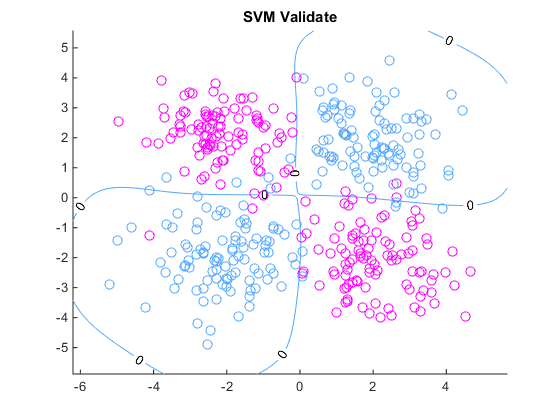
\includegraphics[width=\linewidth]{figures/C,01sigma1.png}
  \caption{$C = 0.01, \sigma = 1$}
\endminipage\hfill
\minipage{0.32\textwidth}
  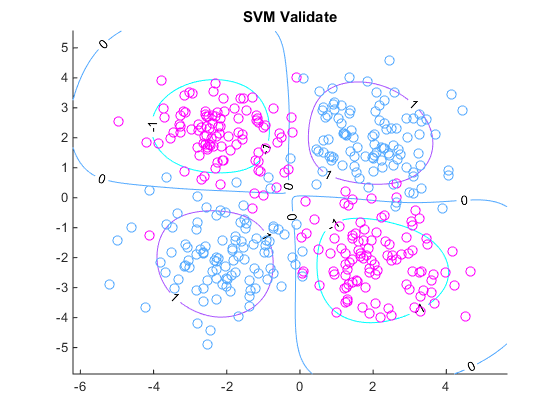
\includegraphics[width=\linewidth]{figures/C,1sigma1.png}
  \caption{$C = 0.1, \sigma = 1$}
\endminipage\hfill
\minipage{0.32\textwidth}
  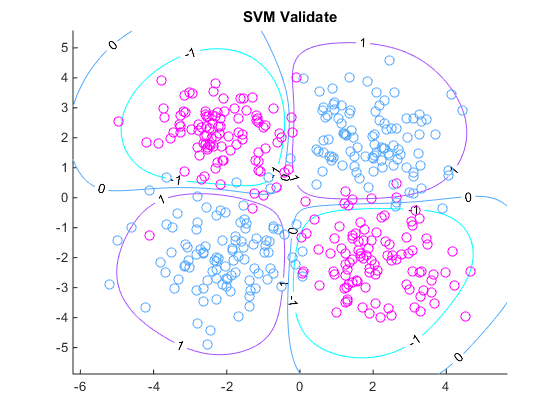
\includegraphics[width=\linewidth]{figures/C1sigma1.png}
  \caption{$C = 1, \sigma = 1$}
\endminipage
\end{figure}
\begin{figure}[!htb]
\hspace{.16\textwidth}
\minipage{0.32\textwidth}
  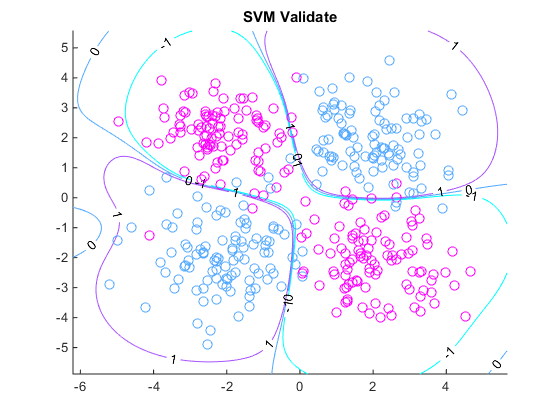
\includegraphics[width=\linewidth]{figures/C10sigma1.png}
  \caption{$C = 10, \sigma = 1$}
\endminipage
\minipage{0.32\textwidth}
  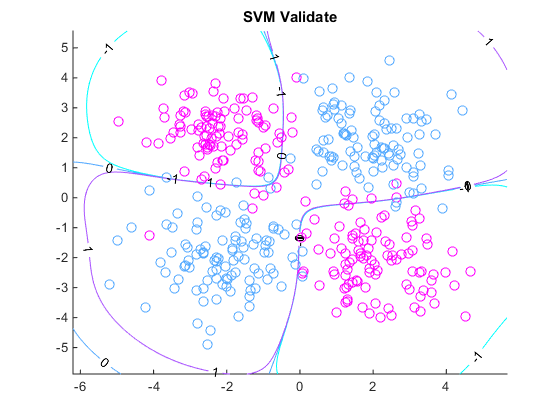
\includegraphics[width=\linewidth]{figures/C100sigma1.png}
  \caption{$C = 100, \sigma = 1$}
\endminipage
\end{figure}
\end{center}

We also note that as $C$ increases, the number of boundary points decreases. Thus, the number of support vectors decrease. For the nonseparable example, for $C = (.01, .1, 1, 10, 100)$, we see that $\mathcal{M} = (400, 324, 133, 68, 59)$.

As per the usual procedure with the approximately equivalent $\lambda$, to select the correct $C$, we first compute $\alpha$ for various values of $C$ using a training set, then determine the validation error using a validation set. We select the $C$ which produces the lowest validation error in order to maximize the generality of our solution.

\end{document}













